\apendice{Plan de Proyecto Software}
\section{Introducción}
La fase de planificación de un proyecto es una de las fase clave cuando se quiere organizar el desarrollo de un proyecto. A grandes rasgos, se exponen las ideas a desarrollar teniendo en cuenta las limitaciones temporales y económicas que exigía el proyecto y la organización.

Este anexo será dividido en dos subapartados:
\begin{itemize}
  \item \textbf{Planificación temporal}: Especifica el formato y contenido de los planes para la gestión de un proyecto \textit{software}.
  \item \textbf{Estudio de viabilidad}: Permite hacer un estudio económico-legal para ver si el proyecto es viable o no. Este subapartado se divide en:
    \begin{itemize}
        \item \underline{Viabilidad económica}: Se hace una estimación de los costes de la aplicación.
        \item \underline{Viabilidad legal}: Se hace un análisis de las tecnologías en base a sus licencias y se tienen en cuenta las leyes actuales en relación al proyecto.
    \end{itemize}
\end{itemize}

\section{Planificación temporal}

Para la realización de este proyecto, la organización \textit{Vicomtech} propuso utilizar \textit{Scrum} como la metodología a utilizar para la realización del proyecto.

Esta metodología divide el trabajo en \textit{Sprints}, siendo la planificación de las tareas a realizar una de las fases mas importantes de esta metodología teniendo en cuenta la duración de cada \textit{sprint}, siendo normalmente de una semana.

\subsection{Sprint 0}

En este primer \textit{sprint} se expusieron, de manera general, todos los aspectos relevantes del proyecto, su arquitectura y cuáles iban a ser los puntos claves del proyecto para su desarrollo. Se investigaron soluciones similares, y posibles tecnologías en el desarrollo del proyecto. 

Este \textit{sprint} duró más de lo habitual, ya que al no conocer ningún aspecto relevante del proyecto y el desconocimiento de algunas de las tecnologías, se tuvo que hacer un gran trabajo de investigación.

\subsection{Sprint 1}

En este \textit{sprint} se decidió que se iba a comenzar por todos los conceptos relacionados con mapas, y sobre su aplicación sobre aplicaciones web en \textit{ReactJs}. Se hizo un trabajo de investigación sobre librerías de mapas para aplicaciones web y sus posibles adaptaciones para la localización \textit{indoor} de usuarios.

Este \textit{sprint} duró mas de lo planificado inicialmente, debido a que las librerías en \textit{Javascript} de mapas no tenían compatibilidad directa con \textit{ReactJs}. Por lo que finalmente se opto por adaptar la importación de la librería \textit{OpenLayers} y utilizar su código en \textit{Javascript vainilla} embebido en código \textit{React}.

\subsection{Sprint 2}

Este \textit{sprint} se basó en utilizar los planos del edificio de la empresa, geolocalizarlo en un \textit{software} llamado \textit{Qgis}, y exportarlo para poderlo utilizar como capa en la librería de mapas web \textit{OpenLayers}.

\subsection{Sprint 3}

En este \textit{sprint} el objetivo se basó en diseñar la \textit{API} que conectaría con la base de datos en archivo \textit{YAML}, para poder generar una versión inicial, en lenguaje \textit{Python} y desplegado en \textit{Docker}, a completar para desarrollar la funcionalidad. Además se implementó un \textit{ORM} de la librería \textit{SQLAlchemy}, para poder interactuar con el contenedor \textit{docker} de la base de datos de manera dinámica en código \textit{Python}.

En cuestiones de funcionalidad, se implementaron parcialmente las funcionalidades de distintos \textit{endpoints}. Pero se dejaron algunas tareas para el siguiente \textit{sprint}.
\begin{figure}[H]
    \centering
    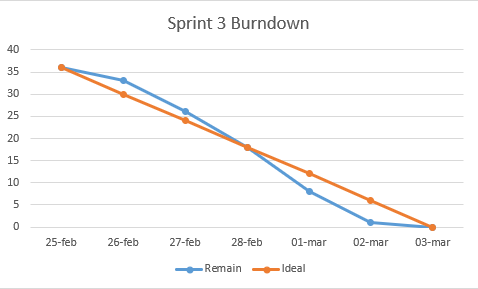
\includegraphics[width=10cm,height=10cm,keepaspectratio]{img/Sprint3_burndow.png}
    \caption{Sprint 3 Burndown.}
    \label{fig:sprint3_burndown}
\end{figure}
\subsection{Sprint 4}

En este sprint el objetivo fue terminar las funcionalidades de los distintos \textit{endpoints} no implementados en el \textit{sprint} anterior, e investigar acerca de las distintas soluciones de \textit{geofencing} existentes para implementar en el proyecto, se eligió \textit{Tile38} como librería \textit{geofencing}.
\begin{figure}[H]
    \centering
    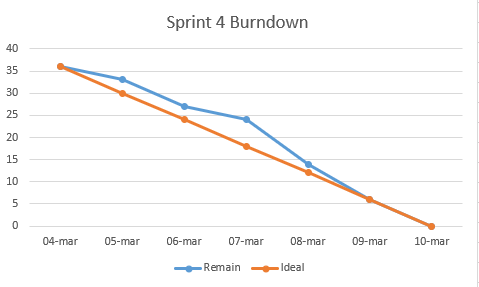
\includegraphics[width=10cm,height=10cm,keepaspectratio]{img/Sprint4_burndow.png}
    \caption{Sprint 4 Burndown.}
    \label{fig:sprint4_burndown}
\end{figure}
\subsection{Sprint 5}

En este Sprint se implementó la librería de los \textit{pyle38} para interactuar con los \textit{dockers} de \textit{Tile38} en la \textit{API} y se trabajó en el \textit{frontend} de la aplicación.
\begin{figure}[H]
    \centering
    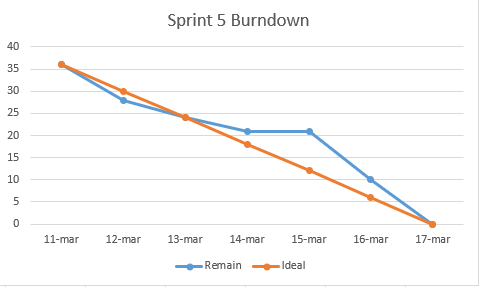
\includegraphics[width=10cm,height=10cm,keepaspectratio]{img/Sprint5_burndow.png}
    \caption{Sprint 5 Burndown.}
    \label{fig:sprint5_burndown}
\end{figure}
\subsection{Sprint 6}
En este \textit{sprint} el objetivo fue trabajar en el \textit{frontend} de la aplicación para poder tener una versión de producción con un buena interfaz de usuario, que genere una buena experiencia de usuario y que no cause confusiones al usuario al utilizar la parte del mapa con otras partes de la aplicación.
\begin{figure}[H]
    \centering
    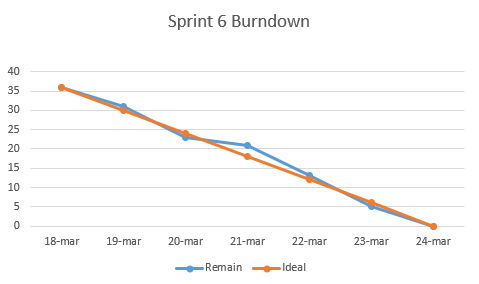
\includegraphics[width=10cm,height=10cm,keepaspectratio]{img/Sprint6_burndow.png}
    \caption{Sprint 6 Burndown.}
    \label{fig:sprint6_burndown}
\end{figure}
\subsection{Sprint 7}
En este \textit{sprint} el objetivo fue documentar toda la aplicación de manera profunda, y ayudar con otras partes del desarrollo a compañeros, así como pulir mis partes de la aplicación y testearla manualmente para su correcto funcionamiento en distintos contextos.

\subsection{Resumen}
En la tabla-resumen se muestran los tiempos dedicados a cada una de las distintas tareas:

\begin{table}[H]
    \setlength{\tabcolsep}{20pt}
    \centering
    \begin{tabular}{@{}l r}
    \noalign{\hrule height 0.8pt}  Categoria &  Tiempo(horas)\\\hline
      Investigación &  47\\
      Desarrollo &  252\\
      Arreglo de errores &  15\\
      Documentación &  70\\
    \hline Total: & 384\\
    \noalign{\hrule height 0.8pt}
    \end{tabular}
    \caption{Tabla recuento de horas de trabajo.}
    \label{tab:Table-counting-working-hours}
\end{table}


\begin{figure}[H]
    \centering
    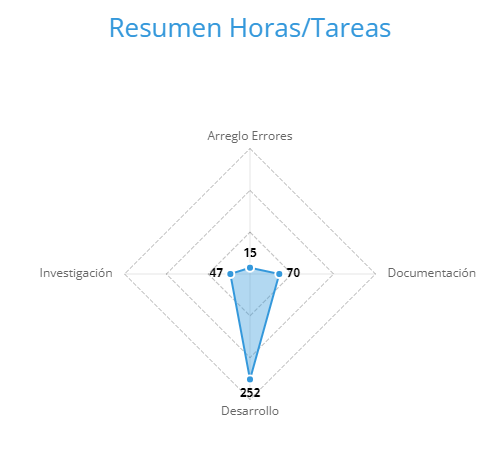
\includegraphics[width=10cm,height=10cm,keepaspectratio]{img/Resumen Horas_Tareas_ (1).png}
    \caption{Gráfico-Resumen horas dedicadas al proyecto.}
    \label{fig:graph-time-working}
\end{figure}
\section{Estudio de viabilidad}
En este punto se hará un análisis desde el punto de vista económica y legal para la viabilidad del proyecto. 
\subsection{Viabilidad económica}
Para la viabilidad económica, se procederán a desglosar los costes que tendrá el desarrollo de la aplicación.

Primero debemos de nombrar los costes del personal que desarrollara la aplicación. Siendo un solo empleado el que realiza la aplicación durante cinco meses el desglose sería:
\FloatBarrier
\begin{table}[h]
    \setlength{\tabcolsep}{20pt}
    \centering
    \begin{tabular}{@{}l r}
    \noalign{\hrule height 0.8pt}  Concepto &  Coste en euros\\\hline
      Salario neto mensual &  1221,75\\
      IRPF(17\%) &  255\\
      Seguridad Social(23,60\%) &  384,44\\
      Salario mensual bruto &  1500\\
    \hline Total 5 meses: & 7500\\
    \noalign{\hrule height 0.8pt}
    \end{tabular}
    \caption{Tabla de coste de personal.}
    \label{tab:table-crew-costs}
\end{table}
\FloatBarrier
Con esto se tendría que hacer un gaste para componentes hardware, quedando otro desglose de:
\FloatBarrier
\begin{table}[h]
    \setlength{\tabcolsep}{20pt}
    \centering
    \begin{tabular}{@{}l r}
    \noalign{\hrule height 0.8pt}  Concepto &  Coste en euros\\\hline
      \textit{MDEK1001 Kit} de desarrollo (12 unidades) &  2456,28\\
      \textit{Rasperry Pi 3} (2 unidades)&  63\\

    \hline Total: & 2519,28\\
    \noalign{\hrule height 0.8pt}
    \end{tabular}
    \caption{Tabla de coste de hardware.}
    \label{tab:table-hardware-costs}
\end{table}
\FloatBarrier
Quedando así la suma de costes totales de la aplicación en:
\FloatBarrier
\begin{table}[h]
    \setlength{\tabcolsep}{20pt}
    \centering
    \begin{tabular}{@{}l r}
    \noalign{\hrule height 0.8pt}  Concepto &  Coste en euros\\\hline
      Personal &  7500\\
      Hardware &  2519,28\\
    \hline Total: & 10019,28\\
    \noalign{\hrule height 0.8pt}
    \end{tabular}
    \caption{Tabla de costes totales.}
    \label{tab:table-total-costs}
\end{table}
\FloatBarrier
Teniendo así que hacer una explotación comercial del \textit{software} para poder recuperar la inversión que se ha hecho en el desarrollo de la aplicación.

\subsection{Viabilidad legal}

Para la explotación comercial del \textit{software} primero se tienen que revisar las licencias legales de las herramientas y librerías utilizadas para el desarrollo de la aplicación.

En esta lista están todas las librerías y herramientas necesarias para la ejecución de la aplicación junto con su correspondiente tipo de licencia:


\FloatBarrier
\begin{table}[h]
    \setlength{\tabcolsep}{5pt}
    \centering
    \begin{tabular}{l p{3cm} p{5cm} p{3cm}}
    Dependencia &  Versión & Descripción & Licencia\\\hline
      Javascript &  ECMAScript 2018 & Lenguaje base de la webapp & CC Atributtion\\
      ReactJS &  17.0 & Framework & MIT\\
      Python &  3.7.0 & Lenguaje API & Python\\
      Flask &  2.0 & Framework API & BSD\\
      SqlAlchemy &  1.4.37 & Librería ORM para conexión con Base de datos & MIT\\
      OpenLayers &  6.14.1 & Librería de Mapas & BSD\\
      JanusWebRTC &  1.0.2 & Librería de \textit{Streaming} de audio y vídeo & GNU\\
    \hline
    \noalign{\hrule height 0.8pt}
    \end{tabular}
    \caption{Tabla dependencias-licencias.}
    \label{tab:table-dependencies-licenses}
\end{table}
\FloatBarrier

Una vez expuestas las licencias de las librerías, la que mas se adapta a nuestro proyecto es \textit{GPLv3} proporcionando derechos de libre uso, de estudio y compartición en copia y la modificación del \textit{software}, informando de los cambios realizados estando bajo la misma licencia.